\documentclass[12pt,a4paper,dvipdfmx]{jsarticle}

\usepackage{amsmath,amssymb}
\usepackage{bm}
\usepackage{here}
\usepackage{ascmac}
\usepackage{xcolor}
\usepackage{listing}
\usepackage{caption}
\usepackage{graphicx}
\usepackage{accsupp}
\usepackage[outputdir=./src]{minted}
\usepackage[utf8]{inputenc}
\usepackage[most, theorems, listings, minted, breakable]{tcolorbox}

\setlength{\textwidth}{\fullwidth}
\setlength{\textheight}{40\baselineskip}
\addtolength{\textheight}{\topskip}
\setlength{\voffset}{-0.2in}
\setlength{\topmargin}{0pt}
\setlength{\headheight}{0pt}
\setlength{\headsep}{0pt}
\usepackage[top=2cm, bottom=2cm, left=2cm, right=2cm]{geometry}

\newcommand{\divergence}{\mathrm{div}\,}  %ダイバージェンス
\newcommand{\grad}{\mathrm{grad}\,}  %グラディエント
\newcommand{\rot}{\mathrm{rot}\,}  %ローテーション

% ignore line number
\newcommand\emptyaccsupp[1]{\BeginAccSupp{ActualText={}}#1\EndAccSupp{}}
\let\theHFancyVerbLine\theFancyVerbLine
\def\theFancyVerbLine{\rmfamily\tiny\emptyaccsupp{\arabic{FancyVerbLine}}}

\definecolor{cite_green}{HTML}{006600}
\renewcommand\thefootnote{\textcolor{red}{\arabic{footnote}}}
\usepackage[dvipdfmx,setpagesize=false,
            colorlinks=true,linkcolor=black,anchorcolor=red,citecolor=cite_green,urlcolor=blue]{hyperref}

\definecolor{bg}{HTML}{333333}
\definecolor{line}{HTML}{000000}

\newenvironment{longlisting}{\captionsetup{type=listing}}{}
\renewcommand\listtablename{表}
\renewcommand\listingscaption{リスト}

\setminted{
    linenos=true,
    autogobble,
}

\newtcblisting[]{myminted}[3][]{%
    theorem={Listing}{listings}{#3}{},
    fonttitle=\scriptsize\bfseries,
    listing engine=minted,
    minted style=monokai,
    minted language=#2,
    colback=bg,
    minted options={%
        linenos,
        breaklines, 
        breakbefore=.,
        autogobble,
        fontsize=\small,
        numbersep=3mm,
        xleftmargin=2mm,
        baselinestretch=1
    },%
    overlay={%
        \begin{tcbclipinterior}
           \fill[gray!25] (frame.south west) rectangle ([xshift=5mm]frame.north west);
        \end{tcbclipinterior}
    },
    breakable,
    enhanced,
    listing only,
    #1,
}%


\title{\LaTeX のtemplate}
\author{高名 典雅}
\date{\today}

\begin{document}
\maketitle
\newcounter{listings}

%\begin{titlepage}

\begin{flushright}
{\large
情報システム実験A
}
\end{flushright}
\begin{center}
\vspace*{200truept}
{\Huge カーネルハック 最終レポート}\\
\vspace{300truept}
{\LARGE 筑波大学 情報学群 情報科学類 3年}\\
\vspace{10truept}
{\LARGE 学籍番号 202213581}\\
\vspace{40truept}
{\huge 高名 典雅}\\
\vspace{40truept}
{\huge 2022年8月5日}\\
\end{center}

\end{titlepage}


\section{概要}
このファイル群は主にレポートに用いられる\LaTeX のテンプレート及び執筆環境である.
これらは,\url{https://github.com/Takana-Norimasa/Latex_template}で管理・公開されている.
以下に忘れやすい数式や表の描き方の例を載せる.

\section{基礎}

\subsection{列挙}
何かを列挙するときは以下.
\begin{itemize}
    \item 酒井桃音
    \item 竹内黄奈子
    \item 浦上紫苑
    \item 河鍋蒼
    \item 菱川翠玉
\end{itemize}

見出しをつけるときは以下.
\begin{itemize}
    \item[書式] void readfile(Words **words,int argc,char **argv);
    \item[概要] ファイルから単語を読み込み構造体の配列に格納する.
    \item[引数] Words **words:単語のリスト.\\
                int argc:実行ファイルの引数の個数.\\
                char **argv:実行ファイルの引数の配列.
    \item[戻り値] なし.
\end{itemize}

数字の列挙は以下.
\begin{enumerate}
  \item item1
  \item item2
  \item ...
  \item itemN
\end{enumerate}


\subsection{表}
表の書き方は以下の通り.
\begin{table}[htb]
    \caption{表の例}
    \label{tab:}
    \centering
    \begin{tabular}{c|c|c}\hline
        & a & b \\\hline\hline
        課題2 & 0.45714286 & 1.74285714\\\hline
        課題3 & 6.03383459 & -5.0112782\\\hline
        課題4 & 0.77429736 & 0.84569739\\\hline
    \end{tabular}
\end{table}

\subsection{図}
図を載せるときは以下.
\begin{figure}[H]
    \centering
    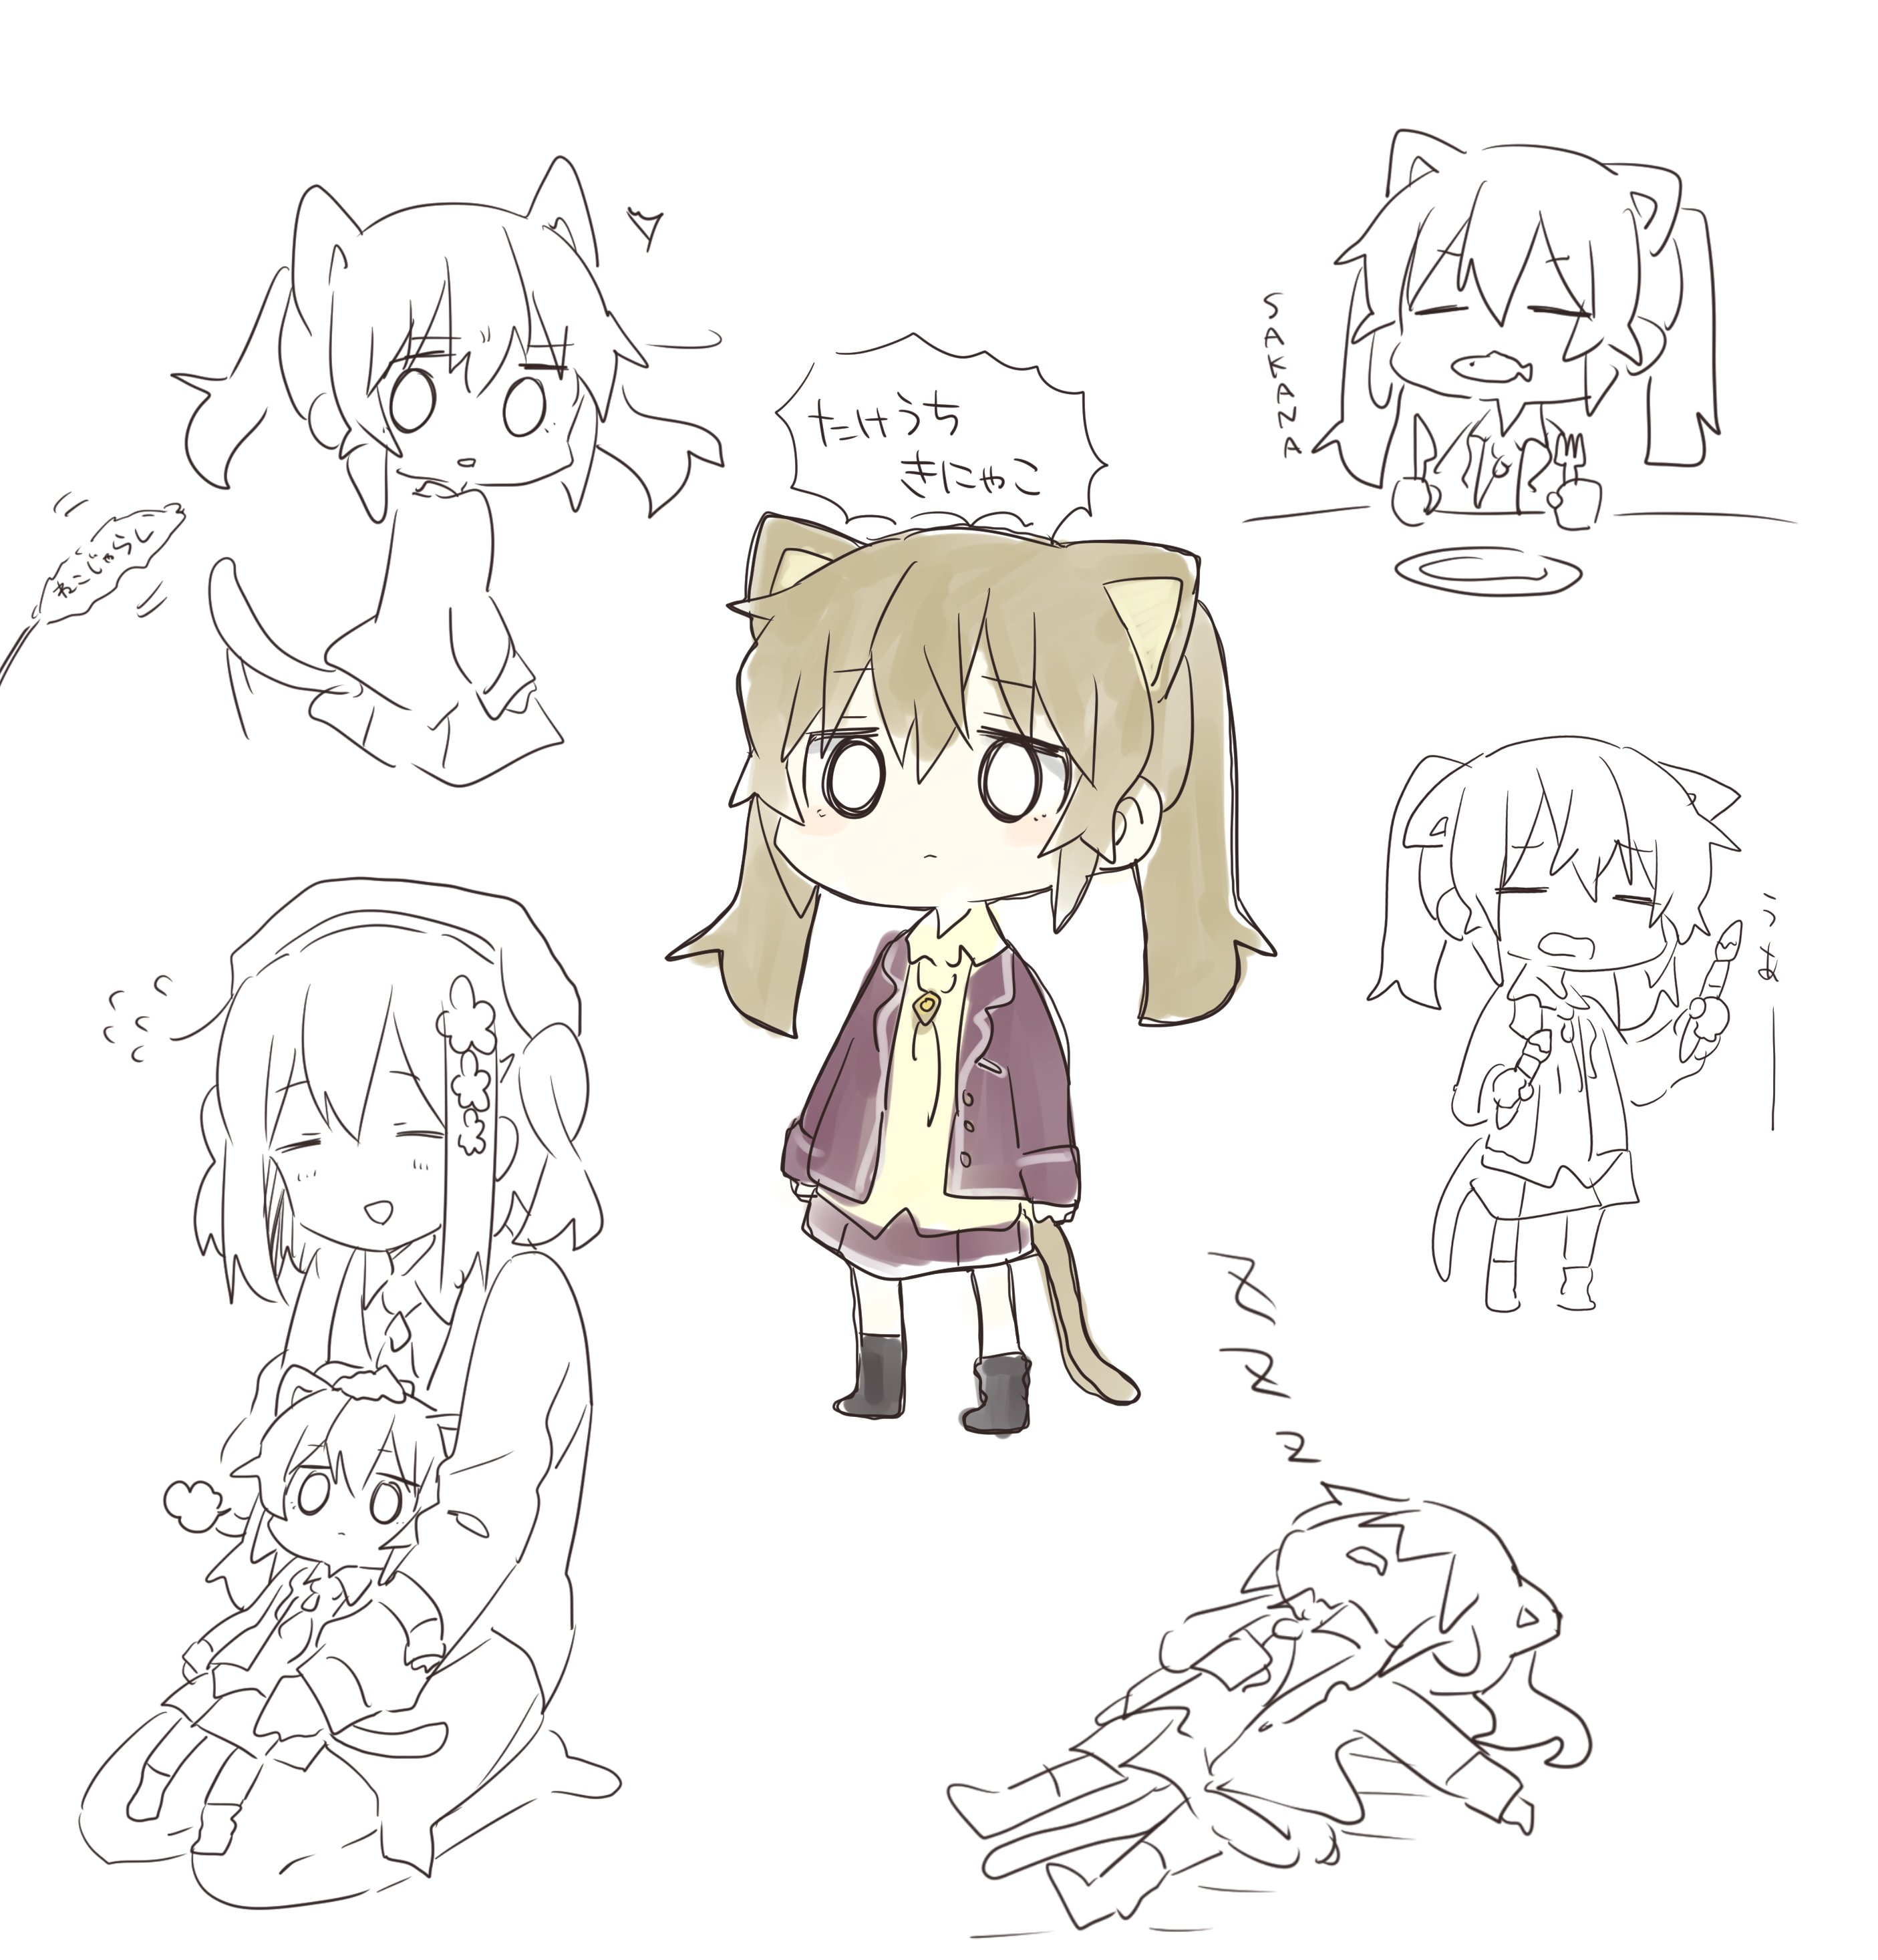
\includegraphics[width=8cm]{./image/Figure_1.png}
    \caption{外部から図を載せる.}
    \label{fig:}
\end{figure}


\subsection{これがsubsection}
これがsubsectionです.
\subsubsection{これがsubsubsection}
これがsubsubsectionです.
\footnote{これがfootnoteです.}

\section{数式}
数式の書き方は以下の通り.

\begin{align*}
    &\sum_{\alpha=1}^{4} x_\alpha y_\alpha = 1\times1 + 2\times3 + 3\times5 + 5\times3 = 1+6+15+15 = 37 \\
    &\pi + \mu - \log_{10} 2 \times \sqrt{x} \div \lim_{h \to 0} \geq \infty
\end{align*}

行列の書き方は以下.
\begin{align*}
        \left(
        \begin{array}{cc}
            a \\
            b
        \end{array}
        \right)
    &=
        \left(
        \begin{array}{cc}
            39 & 11 \\
            11 & 4
        \end{array}
        \right)^{-1}
        \left(
        \begin{array}{cc}
            37 \\
            12
        \end{array}
        \right)
\end{align*}


\section{リスト}
プログラム等を表示したいときは以下.

\begin{longlisting}
\begin{myminted}{cpp}{example}
#include <stdio.h>
#include <omp.h>
#define N 1000000
int main(void){
    int i,j,count0;
    int a[N];
    for(i=0;i<N;i++) a[i]=i%100;
    for(l=0;l<100000;l++){
        coutn0=0;
        #pragma omp parallel for reduction(+:count0) num\_threads(4)
        for(i=0;i<N;i++){
            if(a[i]==0) count0++;
        }
    }
    printf("count0:\%d\n",count0);

    return 0;
}
\end{myminted}
\caption{リストの例}
\label{lst:}
\end{longlisting}

次のページに行くには以下.
\newpage

\section{参考文献}
参考文献はこのように参照する.\cite{bib}

\begin{thebibliography}{9}
    \bibitem{bib} LaTeXコマンド集 - 参考文献,
        \url{http://www.latex-cmd.com/struct/thebibliography.html}
    \bibitem{hou} まんがタイムきららWeb
        \url{http://www.dokidokivisual.com}
    \bibitem{HBD} 桃音のバースデー
        \url{http://www.dokidokivisual.com/doubiju-rt/birthday.html}
    \bibitem{doubiju} どうして私が美術科に!? 1巻 (まんがタイムKRコミックス) | 相崎うたう | Amazon\\
        \url{https://www.amazon.co.jp/dp/B06XFYK4PN}
\end{thebibliography}

\appendix
\section{ここに付録}
プログラムのリストとか.

\end{document}
